
%% bare_conf.tex
%% V1.3
%% 2007/01/11
%% by Michael Shell
%% See:
%% http://www.michaelshell.org/
%% for current contact information.
%%
%% This is a skeleton file demonstrating the use of IEEEtran.cls
%% (requires IEEEtran.cls version 1.7 or later) with an IEEE conference paper.
%%
%% Support sites:
%% http://www.michaelshell.org/tex/ieeetran/
%% http://www.ctan.org/tex-archive/macros/latex/contrib/IEEEtran/
%% and
%% http://www.ieee.org/

%%*************************************************************************
%% Legal Notice:
%% This code is offered as-is without any warranty either expressed or
%% implied; without even the implied warranty of MERCHANTABILITY or
%% FITNESS FOR A PARTICULAR PURPOSE! 
%% User assumes all risk.
%% In no event shall IEEE or any contributor to this code be liable for
%% any damages or losses, including, but not limited to, incidental,
%% consequential, or any other damages, resulting from the use or misuse
%% of any information contained here.
%%
%% All comments are the opinions of their respective authors and are not
%% necessarily endorsed by the IEEE.
%%
%% This work is distributed under the LaTeX Project Public License (LPPL)
%% ( http://www.latex-project.org/ ) version 1.3, and may be freely used,
%% distributed and modified. A copy of the LPPL, version 1.3, is included
%% in the base LaTeX documentation of all distributions of LaTeX released
%% 2003/12/01 or later.
%% Retain all contribution notices and credits.
%% ** Modified files should be clearly indicated as such, including  **
%% ** renaming them and changing author support contact information. **
%%
%% File list of work: IEEEtran.cls, IEEEtran_HOWTO.pdf, bare_adv.tex,
%%                    bare_conf.tex, bare_jrnl.tex, bare_jrnl_compsoc.tex
%%*************************************************************************

% *** Authors should verify (and, if needed, correct) their LaTeX system  ***
% *** with the testflow diagnostic prior to trusting their LaTeX platform ***
% *** with production work. IEEE's font choices can trigger bugs that do  ***
% *** not appear when using other class files.                            ***
% The testflow support page is at:
% http://www.michaelshell.org/tex/testflow/



% Note that the a4paper option is mainly intended so that authors in
% countries using A4 can easily print to A4 and see how their papers will
% look in print - the typesetting of the document will not typically be
% affected with changes in paper size (but the bottom and side margins will).
% Use the testflow package mentioned above to verify correct handling of
% both paper sizes by the user's LaTeX system.
%
% Also note that the "draftcls" or "draftclsnofoot", not "draft", option
% should be used if it is desired that the figures are to be displayed in
% draft mode.
%
\documentclass[conference]{IEEEtran}
\usepackage{blindtext, graphicx}
% Add the compsoc option for Computer Society conferences.
%
% If IEEEtran.cls has not been installed into the LaTeX system files,
% manually specify the path to it like:
% \documentclass[conference]{../sty/IEEEtran}

\usepackage{import}
\usepackage{xcolor}
\usepackage[utf8]{inputenc}
\usepackage{algorithm}
\usepackage[noend]{algpseudocode}
\usepackage{amsmath}
\usepackage{pgfplots}

% Should either be Production or Release
\def \paperstate {Release}

\newcounter{countertodo}
\newcommand{\todo}[1]{
	\stepcounter{countertodo}
	\ifthenelse{\equal{\paperstate}{Production}}{
		[\textcolor{red}{\textbf{\textit{#1}}}]
		\label{todo:#1}
	}{}
}

\newcommand*\ifcounter[1]{%
  \ifcsname c@#1\endcsname
    \expandafter\@firstoftwo
  \else
    \expandafter\@secondoftwo
  \fi
}

\newcommand{\abbrev}[1]{\ifcsname c@counterab#1\endcsname\stepcounter{counterab#1}#1\else\newcounter{counterab#1}(#1)\fi}

\newcommand{\getabbrev}[1]{
	The abbrevation #1 is used \the\numexpr\value{counterab#1}\, times.
}

% Some very useful LaTeX packages include:
% (uncomment the ones you want to load)


% *** MISC UTILITY PACKAGES ***
%
%\usepackage{ifpdf}
% Heiko Oberdiek's ifpdf.sty is very useful if you need conditional
% compilation based on whether the output is pdf or dvi.
% usage:
% \ifpdf
%   % pdf code
% \else
%   % dvi code
% \fi
% The latest version of ifpdf.sty can be obtained from:
% http://www.ctan.org/tex-archive/macros/latex/contrib/oberdiek/
% Also, note that IEEEtran.cls V1.7 and later provides a builtin
% \ifCLASSINFOpdf conditional that works the same way.
% When switching from latex to pdflatex and vice-versa, the compiler may
% have to be run twice to clear warning/error messages.






% *** CITATION PACKAGES ***
%
\usepackage{cite}
% cite.sty was written by Donald Arseneau
% V1.6 and later of IEEEtran pre-defines the format of the cite.sty package
% \cite{} output to follow that of IEEE. Loading the cite package will
% result in citation numbers being automatically sorted and properly
% "compressed/ranged". e.g., [1], [9], [2], [7], [5], [6] without using
% cite.sty will become [1], [2], [5]--[7], [9] using cite.sty. cite.sty's
% \cite will automatically add leading space, if needed. Use cite.sty's
% noadjust option (cite.sty V3.8 and later) if you want to turn this off.
% cite.sty is already installed on most LaTeX systems. Be sure and use
% version 4.0 (2003-05-27) and later if using hyperref.sty. cite.sty does
% not currently provide for hyperlinked citations.
% The latest version can be obtained at:
% http://www.ctan.org/tex-archive/macros/latex/contrib/cite/
% The documentation is contained in the cite.sty file itself.






% *** GRAPHICS RELATED PACKAGES ***
%
\ifCLASSINFOpdf
  % \usepackage[pdftex]{graphicx}
  % declare the path(s) where your graphic files are
  % \graphicspath{{../pdf/}{../jpeg/}}
  % and their extensions so you won't have to specify these with
  % every instance of \includegraphics
  % \DeclareGraphicsExtensions{.pdf,.jpeg,.png}
\else
  % or other class option (dvipsone, dvipdf, if not using dvips). graphicx
  % will default to the driver specified in the system graphics.cfg if no
  % driver is specified.
  % \usepackage[dvips]{graphicx}
  % declare the path(s) where your graphic files are
  % \graphicspath{{../eps/}}
  % and their extensions so you won't have to specify these with
  % every instance of \includegraphics
  % \DeclareGraphicsExtensions{.eps}
\fi
% graphicx was written by David Carlisle and Sebastian Rahtz. It is
% required if you want graphics, photos, etc. graphicx.sty is already
% installed on most LaTeX systems. The latest version and documentation can
% be obtained at: 
% http://www.ctan.org/tex-archive/macros/latex/required/graphics/
% Another good source of documentation is "Using Imported Graphics in
% LaTeX2e" by Keith Reckdahl which can be found as epslatex.ps or
% epslatex.pdf at: http://www.ctan.org/tex-archive/info/
%
% latex, and pdflatex in dvi mode, support graphics in encapsulated
% postscript (.eps) format. pdflatex in pdf mode supports graphics
% in .pdf, .jpeg, .png and .mps (metapost) formats. Users should ensure
% that all non-photo figures use a vector format (.eps, .pdf, .mps) and
% not a bitmapped formats (.jpeg, .png). IEEE frowns on bitmapped formats
% which can result in "jaggedy"/blurry rendering of lines and letters as
% well as large increases in file sizes.
%
% You can find documentation about the pdfTeX application at:
% http://www.tug.org/applications/pdftex





% *** MATH PACKAGES ***
%
%\usepackage[cmex10]{amsmath}
% A popular package from the American Mathematical Society that provides
% many useful and powerful commands for dealing with mathematics. If using
% it, be sure to load this package with the cmex10 option to ensure that
% only type 1 fonts will utilized at all point sizes. Without this option,
% it is possible that some math symbols, particularly those within
% footnotes, will be rendered in bitmap form which will result in a
% document that can not be IEEE Xplore compliant!
%
% Also, note that the amsmath package sets \interdisplaylinepenalty to 10000
% thus preventing page breaks from occurring within multiline equations. Use:
%\interdisplaylinepenalty=2500
% after loading amsmath to restore such page breaks as IEEEtran.cls normally
% does. amsmath.sty is already installed on most LaTeX systems. The latest
% version and documentation can be obtained at:
% http://www.ctan.org/tex-archive/macros/latex/required/amslatex/math/





% *** SPECIALIZED LIST PACKAGES ***
%
%\usepackage{algorithmic}
% algorithmic.sty was written by Peter Williams and Rogerio Brito.
% This package provides an algorithmic environment fo describing algorithms.
% You can use the algorithmic environment in-text or within a figure
% environment to provide for a floating algorithm. Do NOT use the algorithm
% floating environment provided by algorithm.sty (by the same authors) or
% algorithm2e.sty (by Christophe Fiorio) as IEEE does not use dedicated
% algorithm float types and packages that provide these will not provide
% correct IEEE style captions. The latest version and documentation of
% algorithmic.sty can be obtained at:
% http://www.ctan.org/tex-archive/macros/latex/contrib/algorithms/
% There is also a support site at:
% http://algorithms.berlios.de/index.html
% Also of interest may be the (relatively newer and more customizable)
% algorithmicx.sty package by Szasz Janos:
% http://www.ctan.org/tex-archive/macros/latex/contrib/algorithmicx/




% *** ALIGNMENT PACKAGES ***
%
%\usepackage{array}
% Frank Mittelbach's and David Carlisle's array.sty patches and improves
% the standard LaTeX2e array and tabular environments to provide better
% appearance and additional user controls. As the default LaTeX2e table
% generation code is lacking to the point of almost being broken with
% respect to the quality of the end results, all users are strongly
% advised to use an enhanced (at the very least that provided by array.sty)
% set of table tools. array.sty is already installed on most systems. The
% latest version and documentation can be obtained at:
% http://www.ctan.org/tex-archive/macros/latex/required/tools/


%\usepackage{mdwmath}
%\usepackage{mdwtab}
% Also highly recommended is Mark Wooding's extremely powerful MDW tools,
% especially mdwmath.sty and mdwtab.sty which are used to format equations
% and tables, respectively. The MDWtools set is already installed on most
% LaTeX systems. The lastest version and documentation is available at:
% http://www.ctan.org/tex-archive/macros/latex/contrib/mdwtools/


% IEEEtran contains the IEEEeqnarray family of commands that can be used to
% generate multiline equations as well as matrices, tables, etc., of high
% quality.


%\usepackage{eqparbox}
% Also of notable interest is Scott Pakin's eqparbox package for creating
% (automatically sized) equal width boxes - aka "natural width parboxes".
% Available at:
% http://www.ctan.org/tex-archive/macros/latex/contrib/eqparbox/





% *** SUBFIGURE PACKAGES ***
%\usepackage[tight,footnotesize]{subfigure}
% subfigure.sty was written by Steven Douglas Cochran. This package makes it
% easy to put subfigures in your figures. e.g., "Figure 1a and 1b". For IEEE
% work, it is a good idea to load it with the tight package option to reduce
% the amount of white space around the subfigures. subfigure.sty is already
% installed on most LaTeX systems. The latest version and documentation can
% be obtained at:
% http://www.ctan.org/tex-archive/obsolete/macros/latex/contrib/subfigure/
% subfigure.sty has been superceeded by subfig.sty.



%\usepackage[caption=false]{caption}
%\usepackage[font=footnotesize]{subfig}
% subfig.sty, also written by Steven Douglas Cochran, is the modern
% replacement for subfigure.sty. However, subfig.sty requires and
% automatically loads Axel Sommerfeldt's caption.sty which will override
% IEEEtran.cls handling of captions and this will result in nonIEEE style
% figure/table captions. To prevent this problem, be sure and preload
% caption.sty with its "caption=false" package option. This is will preserve
% IEEEtran.cls handing of captions. Version 1.3 (2005/06/28) and later 
% (recommended due to many improvements over 1.2) of subfig.sty supports
% the caption=false option directly:
%\usepackage[caption=false,font=footnotesize]{subfig}
%
% The latest version and documentation can be obtained at:
% http://www.ctan.org/tex-archive/macros/latex/contrib/subfig/
% The latest version and documentation of caption.sty can be obtained at:
% http://www.ctan.org/tex-archive/macros/latex/contrib/caption/




% *** FLOAT PACKAGES ***
%
%\usepackage{fixltx2e}
% fixltx2e, the successor to the earlier fix2col.sty, was written by
% Frank Mittelbach and David Carlisle. This package corrects a few problems
% in the LaTeX2e kernel, the most notable of which is that in current
% LaTeX2e releases, the ordering of single and double column floats is not
% guaranteed to be preserved. Thus, an unpatched LaTeX2e can allow a
% single column figure to be placed prior to an earlier double column
% figure. The latest version and documentation can be found at:
% http://www.ctan.org/tex-archive/macros/latex/base/



%\usepackage{stfloats}
% stfloats.sty was written by Sigitas Tolusis. This package gives LaTeX2e
% the ability to do double column floats at the bottom of the page as well
% as the top. (e.g., "\begin{figure*}[!b]" is not normally possible in
% LaTeX2e). It also provides a command:
%\fnbelowfloat
% to enable the placement of footnotes below bottom floats (the standard
% LaTeX2e kernel puts them above bottom floats). This is an invasive package
% which rewrites many portions of the LaTeX2e float routines. It may not work
% with other packages that modify the LaTeX2e float routines. The latest
% version and documentation can be obtained at:
% http://www.ctan.org/tex-archive/macros/latex/contrib/sttools/
% Documentation is contained in the stfloats.sty comments as well as in the
% presfull.pdf file. Do not use the stfloats baselinefloat ability as IEEE
% does not allow \baselineskip to stretch. Authors submitting work to the
% IEEE should note that IEEE rarely uses double column equations and
% that authors should try to avoid such use. Do not be tempted to use the
% cuted.sty or midfloat.sty packages (also by Sigitas Tolusis) as IEEE does
% not format its papers in such ways.





% *** PDF, URL AND HYPERLINK PACKAGES ***
%
%\usepackage{url}
% url.sty was written by Donald Arseneau. It provides better support for
% handling and breaking URLs. url.sty is already installed on most LaTeX
% systems. The latest version can be obtained at:
% http://www.ctan.org/tex-archive/macros/latex/contrib/misc/
% Read the url.sty source comments for usage information. Basically,
% \url{my_url_here}.





% *** Do not adjust lengths that control margins, column widths, etc. ***
% *** Do not use packages that alter fonts (such as pslatex).         ***
% There should be no need to do such things with IEEEtran.cls V1.6 and later.
% (Unless specifically asked to do so by the journal or conference you plan
% to submit to, of course. )


% correct bad hyphenation here
\hyphenation{op-tical net-works semi-conduc-tor}


\begin{document}
%
% paper title
% can use linebreaks \\ within to get better formatting as desired
\title{Learning human motion features and trajectory predictions in large changing environments}


% author names and affiliations
% use a multiple column layout for up to three different
% affiliations
\author{\IEEEauthorblockN{Robin Eberhard, Stefan Dörr}
%\and
%\IEEEauthorblockN{Stefan Dörr}
}

% conference papers do not typically use \thanks and this command
% is locked out in conference mode. If really needed, such as for
% the acknowledgment of grants, issue a \IEEEoverridecommandlockouts
% after \documentclass

% for over three affiliations, or if they all won't fit within the width
% of the page, use this alternative format:
% 
%\author{\IEEEauthorblockN{Michael Shell\IEEEauthorrefmark{1},
%Homer Simpson\IEEEauthorrefmark{2},
%James Kirk\IEEEauthorrefmark{3}, 
%Montgomery Scott\IEEEauthorrefmark{3} and
%Eldon Tyrell\IEEEauthorrefmark{4}}
%\IEEEauthorblockA{\IEEEauthorrefmark{1}School of Electrical and Computer Engineering\\
%Georgia Institute of Technology,
%Atlanta, Georgia 30332--0250\\ Email: see http://www.michaelshell.org/contact.html}
%\IEEEauthorblockA{\IEEEauthorrefmark{2}Twentieth Century Fox, Springfield, USA\\
%Email: homer@thesimpsons.com}
%\IEEEauthorblockA{\IEEEauthorrefmark{3}Starfleet Academy, San Francisco, California 96678-2391\\
%Telephone: (800) 555--1212, Fax: (888) 555--1212}
%\IEEEauthorblockA{\IEEEauthorrefmark{4}Tyrell Inc., 123 Replicant Street, Los Angeles, California 90210--4321}}




% use for special paper notices
%\IEEEspecialpapernotice{(Invited Paper)}




% make the title area
\maketitle


\begin{abstract}
%\boldmath

This study presents a new approach to detecting humans in service environments. Making use of the latest advances in neural networks, fast scalable applications can be modeled without having knowledge about the inner workings. We present a leg detection tool, that operates only on laser scan data, classifying each point as human or non-human. The results are further used to learn to identify people, allowing for precise operation of an autonomous robot in the service industry. This also includes prediction of trajectories, which will be used for movement in crowded scenes.


\end{abstract}



% IEEEtran.cls defaults to using nonbold math in the Abstract.
% This preserves the distinction between vectors and scalars. However,
% if the journal you are submitting to favors bold math in the abstract,
% then you can use LaTeX's standard command \boldmath at the very start
% of the abstract to achieve this. Many IEEE journals frown on math
% in the abstract anyway.

% Note that keywords are not normally used for peerreview papers.
\begin{IEEEkeywords}
\todo{keywords}.
\end{IEEEkeywords}






% For peer review papers, you can put extra information on the cover
% page as needed:
% \ifCLASSOPTIONpeerreview
% \begin{center} \bfseries EDICS Category: 3-BBND \end{center}
% \fi
%
% For peerreview papers, this IEEEtran command inserts a page break and
% creates the second title. It will be ignored for other modes.
\IEEEpeerreviewmaketitle
\section{Introduction}

Autonomous robots are making their way from the production industry to the service industry. This change introduces a new set of problems, that deal with interactions of people and robots. These could include for example following and approaching customers, and navigating through a crowded environment. 

To solve these problems, the first step is the detection of people, which is here done using a safety laser detector on leg-height\footnote{Sick S300 safety laser scanner}. In the past, this has already been approached with model-based solutions, that require prior knowledge about shapes and behaviour of legs \cite{Arras07usingboosted} \cite{weinrich2014people}.
We present a new approach, where a neural network learns characteristics on its own and places unique identifiers on persons, making it easy to track them over a long period of time.

Having the information and history of positions of people, we can learn trajectories, behaviour and intentions when the robot is serving customers. We provide a way to model the trajectories using Long short-term memory (LSTM) cells in combination with a Mixture density layer, which outputs a set of normal distributions, similar to \cite{bishop1994mixture} \cite{graves2013generating}.

In this paper, we present the models that are used to train the program, as well as some benchmarking and comparisons with similar projects.
\section{State of the art}

Lidar scanners pose an attractive way to scan the environment, due to the simple interpretation of the data and the low computational power required.
The idea to extract people from this input has been introduced in \cite{1013691} where laser range measurements are grouped into blobs and objects. 
Moving objects are considered as people with the downside of not detecting immovable objects.
In order to improve on this idea, a combination of Lidar and vision data \cite{kleinehagenbrock2002person} can be applied. Information of leg positions are here extracted from the laser scanner, while a camera provides additional information through skin-colored face detection. 
Arras et al. proposed a machine learning algorithm \cite{Arras07usingboosted}, where pre-defined geometrical features are trained in a supervised learning approach. 
It was further adapted in \cite{weinrich2014people} to expand the detection in retirement homes, allowing the classification of people with different walking aids. 
The algorithm allows to add additional features, which are weighted and therefore filtered by importance.
However, the expert knowledge of geometrical features pose a downside to the algorithm as well as the computational power required during evaluation. Convolutional neural networks therefore present a way to learn features without prior expertise. Since their introduction \cite{lecun_gradient-based_1998}, they are the go-to standard for object detection \cite{krizhevsky_imagenet_2012}, due to their versatility and their simple and fast implementation. Convolutional networks can be further expanded for segmentation of images \cite{long2015fully}, which gives a way to keep the input dimensionality while simultaneously detect and label objects.

Trajectory prediction has already been achieved in \cite{graves2013generating}, where handwriting is generated using a mixture density network (MDN) \cite{bishop1994mixture}. These networks provide a way to model the most probable outcome as a function of multiple density terms. In order to predict from a history of input values, a Long short term memory (LSTM) \cite{hochreiter1997long} is included. This allows a way to store previous inputs and therefore predict outcomes when similarities are found. People based trajectory prediction has previously been achieved \cite{alahi2016social} using a similar approach. Making use of LSTM and MDN we therefore predict trajectories using unsupervised learning, requiring only positions of people as an input.
\section{Model architecture}
\label{sec:model_arch}

\label{sec:Model}

Learning to detect people from laser scans requires a neural network to solve several tasks. 
First, each laser scan point has to be classified as leg or non-leg.
This task is solved by using a set of convolutional and pooling layers. 
The points labeled as belonging to legs are sorted out and clustered in order to identify persons.
In a naive approach, this clustering is carried out based on euclidian distance between scan points.
However, this approach does not work well, when people are close to each other or when they are moving, as the algorithm would then either cluster too many legs together or see two legs as separate people respectively.

This can be countered by supplying the clustering algorithm with additional information.
During the convolution step, the network learns features which are unique to legs in different situations. 
Those can be extracted and passed as additional parameters to the clustering algorithm, which not only allows higher accuracy, but also providing a pair of legs with a unique identifier.

Having identifiers and positions, they can then be fed into the third and last step of the setup, which aims to predict trajectories of individual people. The network takes a set of positions, that are run through an LSTM cell, which implicitly works as a memory for the program and holds the information necessary to build future trajectories.

\subsection{Classification of the lidar data}
\label{sec:classification}

\begin{figure}

\def\svgwidth{0.4 \textwidth}
\small
\import{figures/}{conv_layers.pdf_tex}
\caption{\textbf{Lidar classification.} (1) The input is a 2D array of $N_{points} \times N_{frames}$ containing distances from a laser scan. It is fed into (2), where features are extracted using convolutions and downscaled using a pooling layer. After $N_{conv}$ iterations of (2), the now one-dimensional output is upscaled in (3) into the shape $N_{points}$. (4) multiplies the output and applies the softmax function, resulting in probabilities of each point belonging to class leg or non-leg in (5).}
\label{fig:laser_classification}
\end{figure}

In order to classify a lidar data, a snapshot of the current scan is taken in equal timesteps. Each snapshot contains one dimensional arrays of length $N_{points}$ with distances $r_i$ to the closest intersections from the laser beams.

From the one-dimensional array as input, the network would only find characteristics in the objective shapes of the laser scans. To also account for movement, $N_{frames}$ snapshots are composed together.
The desired outputs are probabilities for each point in the most current snapshot to be in either class leg or non-leg.

Therefore, the mathematical description of the model can be described by a function $F$ that maps an input of size $[N_{frames}, N_{points}]$ to an output of size $[N_{points}, 2]$.

The output is modelled from the input as outlined in Figure \ref{fig:laser_classification} and described in more detail in the following.
When convolutional layers are used for classification, a network will train the weights such that they represent characteristics for a class. In this way, the characteristics are first of geometrical nature and become more abstract the more layers there are.

The input is therefore fed into a convolutional layer and then downsampled using a max pooling layer. This is repeated $N_{conv}$ times, after which the output is a one dimensional array of length smaller than $N_{points}$.

To gain a classification for each point in the most current laser scan, the output is upscaled using transpose convolutions, again extracting features. Multiplication by output weights and applying the softmax function results in the desired shape $[N_{points}, 2]$. Each entry consists of the two probabilities of a point being in class leg $P_{leg}$ or non-leg $P_{nonleg}$ with $P_{leg} + P_{nonleg} = 1$.



\subsection{Clustering of leg points}
\label{subs:clustering}

In order to gain information about the legs position and identity people, the classified points are clustered. This usually poses two major problems:
\begin{itemize}
\item The clustering has a high margin of error when legs of a single person are too far away or when legs of different people are close to each other.
\item The tracking of a person has to be handled externally.
\end{itemize} 
With the following approach, we find a high accuracy and are also able to track people on certain features.

As the inputs are convoluted, the network finds characteristics, such as shapes and movement. In order to find the most important characteristics, a training was implemented to find weights $v$, such that parameters of people in different situations are easily separable. The $i$th convoluted layer has its weights $w_i$ multiplied by $v_i$ and the resulting cluster parameter $p_i$ is then found by the sum of all weights:
\begin{equation}
	p_i = v_{i} * \sum_{j} w_{i,j}
\end{equation}

This introduces $2*N_{convs}$ additional parameters to the clustering algorithm, highly increasing accuracy when used together with the euclidian distance. As the parameters have been chosen such that people in different situations are easily separable and given the unlikeliness of two people being in the same position in the same situation, we can additionally use the parameters to place a similar identifier on a single person over several frames. This allows to track them in order to predict their movements.

\begin{figure}
% Hier kannst du einstellen, wie groß das Bild in deinem Dokument ist (der Text wird nicht mit skaliert)
\def\svgwidth{0.4 \textwidth}
% Hier die schriftgröße im Bild
\small
% Der Pfad zu der pdf_tex Datei
\import{figures/}{cluster_convs.pdf_tex}
% Hier ne Bildunterschrift
\caption{\textbf{Convolution-based clustering.} (1) For every point in the current laser scan, $N_{conv}$ convolutions are created. A clustering parameter $p_i$ is derived from the weights $w_i$ of the convolution and the trained weights $v_i$, which assumes that some convolutions are more important than others. (2) The resulting clustering matrix holds $n=2*N_{conv}$ parameters for each point in the current laser scan.}
\label{fig:cluster_convs}
\end{figure}




\subsection{Trajectory prediction}

With the information about the position of individual persons, we can learn to predict trajectories over some time horizon. A trajectory of a single person can be modeled with a normal distribution, or if the path is unclear, a number of distributions $N_{dist}$ are necessary.

This leads to the approach of using a mixture density network \cite{bishop1994mixture}. The network learns from parameters $\pi$, $\mu$, $\sigma$ and $\rho$ according to \cite{graves2013generating}, so that a distribution is given as:
\begin{equation}
	\mathcal{N}(x|\mu,\sigma,\rho) = \frac{1}{2\pi\sigma_1\sigma_2\sqrt{1-\rho^2}} \exp\left[ \frac{-Z}{2(1-\rho^2)} \right]
\end{equation}
with
\begin{equation}
	Z = \frac{(x_1 - \mu_1)^2}{\sigma_1^2} + \frac{(x_2 - \mu_2)^2}{\sigma_2^2} - \frac{2\rho(x_1-\mu_1)(x_2-\mu_2)}{\sigma_1\sigma_2}.
\end{equation}
Therefore we can define the ensemble of distributions as
\begin{equation}
	Pr(x|y) = \sum_{j=1}^{N_{dist}} \pi_j \mathcal{N}(x|\mu_j,\sigma_j,\rho_j)
\end{equation}
for every input point $x$ from the laser scan.

As the future movement depends on previous positions, the parameters $\mu$, $\sigma$, $\rho$ and $\pi$ are derived from a recurrent network cell. A LSTM was used, which allows for information to be kept over a long time. This way, the network was trained on different patterns, so that it can recognize similar ones later in the evaluation. The LSTM cell will take the input positions and directly outputs the parameters for the mixture of normal distributions.
\section{Experimental results}
\label{sec:Experiment}

\subsection{Classification of lidar data}

The leg detector was trained as described in \ref{sec:classification}, using labeled data from various sources. These include data from \cite{Arras07usingboosted}, \cite{weinrich2014people} as well as custom data from a laboratory and a retail environment, where people interacted more extensively with the robot.
In order to evaluate the leg detector, the robot was set up in a corridor, recording legs of people passing through over a course of three hours. Walls were separated from the passage, which results in labeled laser measurements, which are compared to the detector in order to evaluate its accuracy. The leg detector receives the input from the laser scan and labels each point as leg or non-leg.
In the comparison to the ground truth, we find, that the detector works best in close range, while becoming weaker as the range increases. This is demonstrated in Figure \ref{fig:radius_detection}, where a short, 100 second long exposure was analyzed.

The decrease in the first half originates mainly from the difficulty of interpreting the laser data, as the points spread further out depending on the distance to the scanner. The second half additionally suggests too few data points as input to the convolutional network and the clustering algorithm, which ultimately decides the outcome.
At a distance of $2.2 m$ we still find good results in a reasonable range around the robot, which we can use to evaluate a three hour long recording of the same corridor. We find the confusion matrix in Table \ref{tab:truth}, omitting false and true negatives as the sensor recorded only a specific wall in that range as negative data, making the input redundant. The long recording shows how well the network reacts to more arbitrary data, most importantly the accuracy is still high, which we can compare against the state of the art leg detector.

\begin{figure}[]
	\normalsize
	\begin{center}
		%% Creator: Matplotlib, PGF backend
%%
%% To include the figure in your LaTeX document, write
%%   \input{<filename>.pgf}
%%
%% Make sure the required packages are loaded in your preamble
%%   \usepackage{pgf}
%%
%% Figures using additional raster images can only be included by \input if
%% they are in the same directory as the main LaTeX file. For loading figures
%% from other directories you can use the `import` package
%%   \usepackage{import}
%% and then include the figures with
%%   \import{<path to file>}{<filename>.pgf}
%%
%% Matplotlib used the following preamble
%%   \usepackage{fontspec}
%%   \setmainfont{DejaVu Serif}
%%   \setsansfont{DejaVu Sans}
%%   \setmonofont{DejaVu Sans Mono}
%%
\begingroup%
\makeatletter%
\begin{pgfpicture}%
\pgfpathrectangle{\pgfpointorigin}{\pgfqpoint{3.600000in}{2.000000in}}%
\pgfusepath{use as bounding box, clip}%
\begin{pgfscope}%
\pgfsetbuttcap%
\pgfsetmiterjoin%
\definecolor{currentfill}{rgb}{1.000000,1.000000,1.000000}%
\pgfsetfillcolor{currentfill}%
\pgfsetlinewidth{0.000000pt}%
\definecolor{currentstroke}{rgb}{1.000000,1.000000,1.000000}%
\pgfsetstrokecolor{currentstroke}%
\pgfsetdash{}{0pt}%
\pgfpathmoveto{\pgfqpoint{0.000000in}{0.000000in}}%
\pgfpathlineto{\pgfqpoint{3.600000in}{0.000000in}}%
\pgfpathlineto{\pgfqpoint{3.600000in}{2.000000in}}%
\pgfpathlineto{\pgfqpoint{0.000000in}{2.000000in}}%
\pgfpathclose%
\pgfusepath{fill}%
\end{pgfscope}%
\begin{pgfscope}%
\pgfsetbuttcap%
\pgfsetmiterjoin%
\definecolor{currentfill}{rgb}{1.000000,1.000000,1.000000}%
\pgfsetfillcolor{currentfill}%
\pgfsetlinewidth{0.000000pt}%
\definecolor{currentstroke}{rgb}{0.000000,0.000000,0.000000}%
\pgfsetstrokecolor{currentstroke}%
\pgfsetstrokeopacity{0.000000}%
\pgfsetdash{}{0pt}%
\pgfpathmoveto{\pgfqpoint{0.467222in}{0.582778in}}%
\pgfpathlineto{\pgfqpoint{3.415000in}{0.582778in}}%
\pgfpathlineto{\pgfqpoint{3.415000in}{1.435816in}}%
\pgfpathlineto{\pgfqpoint{0.467222in}{1.435816in}}%
\pgfpathclose%
\pgfusepath{fill}%
\end{pgfscope}%
\begin{pgfscope}%
\pgfsetbuttcap%
\pgfsetroundjoin%
\definecolor{currentfill}{rgb}{0.000000,0.000000,0.000000}%
\pgfsetfillcolor{currentfill}%
\pgfsetlinewidth{0.803000pt}%
\definecolor{currentstroke}{rgb}{0.000000,0.000000,0.000000}%
\pgfsetstrokecolor{currentstroke}%
\pgfsetdash{}{0pt}%
\pgfsys@defobject{currentmarker}{\pgfqpoint{0.000000in}{-0.048611in}}{\pgfqpoint{0.000000in}{0.000000in}}{%
\pgfpathmoveto{\pgfqpoint{0.000000in}{0.000000in}}%
\pgfpathlineto{\pgfqpoint{0.000000in}{-0.048611in}}%
\pgfusepath{stroke,fill}%
}%
\begin{pgfscope}%
\pgfsys@transformshift{0.540619in}{0.582778in}%
\pgfsys@useobject{currentmarker}{}%
\end{pgfscope}%
\end{pgfscope}%
\begin{pgfscope}%
\pgftext[x=0.540619in,y=0.485556in,,top]{0}%
\end{pgfscope}%
\begin{pgfscope}%
\pgfsetbuttcap%
\pgfsetroundjoin%
\definecolor{currentfill}{rgb}{0.000000,0.000000,0.000000}%
\pgfsetfillcolor{currentfill}%
\pgfsetlinewidth{0.803000pt}%
\definecolor{currentstroke}{rgb}{0.000000,0.000000,0.000000}%
\pgfsetstrokecolor{currentstroke}%
\pgfsetdash{}{0pt}%
\pgfsys@defobject{currentmarker}{\pgfqpoint{0.000000in}{-0.048611in}}{\pgfqpoint{0.000000in}{0.000000in}}{%
\pgfpathmoveto{\pgfqpoint{0.000000in}{0.000000in}}%
\pgfpathlineto{\pgfqpoint{0.000000in}{-0.048611in}}%
\pgfusepath{stroke,fill}%
}%
\begin{pgfscope}%
\pgfsys@transformshift{1.370663in}{0.582778in}%
\pgfsys@useobject{currentmarker}{}%
\end{pgfscope}%
\end{pgfscope}%
\begin{pgfscope}%
\pgftext[x=1.370663in,y=0.485556in,,top]{2000}%
\end{pgfscope}%
\begin{pgfscope}%
\pgfsetbuttcap%
\pgfsetroundjoin%
\definecolor{currentfill}{rgb}{0.000000,0.000000,0.000000}%
\pgfsetfillcolor{currentfill}%
\pgfsetlinewidth{0.803000pt}%
\definecolor{currentstroke}{rgb}{0.000000,0.000000,0.000000}%
\pgfsetstrokecolor{currentstroke}%
\pgfsetdash{}{0pt}%
\pgfsys@defobject{currentmarker}{\pgfqpoint{0.000000in}{-0.048611in}}{\pgfqpoint{0.000000in}{0.000000in}}{%
\pgfpathmoveto{\pgfqpoint{0.000000in}{0.000000in}}%
\pgfpathlineto{\pgfqpoint{0.000000in}{-0.048611in}}%
\pgfusepath{stroke,fill}%
}%
\begin{pgfscope}%
\pgfsys@transformshift{2.200707in}{0.582778in}%
\pgfsys@useobject{currentmarker}{}%
\end{pgfscope}%
\end{pgfscope}%
\begin{pgfscope}%
\pgftext[x=2.200707in,y=0.485556in,,top]{4000}%
\end{pgfscope}%
\begin{pgfscope}%
\pgfsetbuttcap%
\pgfsetroundjoin%
\definecolor{currentfill}{rgb}{0.000000,0.000000,0.000000}%
\pgfsetfillcolor{currentfill}%
\pgfsetlinewidth{0.803000pt}%
\definecolor{currentstroke}{rgb}{0.000000,0.000000,0.000000}%
\pgfsetstrokecolor{currentstroke}%
\pgfsetdash{}{0pt}%
\pgfsys@defobject{currentmarker}{\pgfqpoint{0.000000in}{-0.048611in}}{\pgfqpoint{0.000000in}{0.000000in}}{%
\pgfpathmoveto{\pgfqpoint{0.000000in}{0.000000in}}%
\pgfpathlineto{\pgfqpoint{0.000000in}{-0.048611in}}%
\pgfusepath{stroke,fill}%
}%
\begin{pgfscope}%
\pgfsys@transformshift{3.030752in}{0.582778in}%
\pgfsys@useobject{currentmarker}{}%
\end{pgfscope}%
\end{pgfscope}%
\begin{pgfscope}%
\pgftext[x=3.030752in,y=0.485556in,,top]{6000}%
\end{pgfscope}%
\begin{pgfscope}%
\pgftext[x=1.941111in,y=0.295587in,,top]{Number of points to label}%
\end{pgfscope}%
\begin{pgfscope}%
\pgfsetbuttcap%
\pgfsetroundjoin%
\definecolor{currentfill}{rgb}{0.000000,0.000000,0.000000}%
\pgfsetfillcolor{currentfill}%
\pgfsetlinewidth{0.803000pt}%
\definecolor{currentstroke}{rgb}{0.000000,0.000000,0.000000}%
\pgfsetstrokecolor{currentstroke}%
\pgfsetdash{}{0pt}%
\pgfsys@defobject{currentmarker}{\pgfqpoint{-0.048611in}{0.000000in}}{\pgfqpoint{0.000000in}{0.000000in}}{%
\pgfpathmoveto{\pgfqpoint{0.000000in}{0.000000in}}%
\pgfpathlineto{\pgfqpoint{-0.048611in}{0.000000in}}%
\pgfusepath{stroke,fill}%
}%
\begin{pgfscope}%
\pgfsys@transformshift{0.467222in}{0.871425in}%
\pgfsys@useobject{currentmarker}{}%
\end{pgfscope}%
\end{pgfscope}%
\begin{pgfscope}%
\pgftext[x=0.149121in,y=0.818664in,left,base]{0.8}%
\end{pgfscope}%
\begin{pgfscope}%
\pgfsetbuttcap%
\pgfsetroundjoin%
\definecolor{currentfill}{rgb}{0.000000,0.000000,0.000000}%
\pgfsetfillcolor{currentfill}%
\pgfsetlinewidth{0.803000pt}%
\definecolor{currentstroke}{rgb}{0.000000,0.000000,0.000000}%
\pgfsetstrokecolor{currentstroke}%
\pgfsetdash{}{0pt}%
\pgfsys@defobject{currentmarker}{\pgfqpoint{-0.048611in}{0.000000in}}{\pgfqpoint{0.000000in}{0.000000in}}{%
\pgfpathmoveto{\pgfqpoint{0.000000in}{0.000000in}}%
\pgfpathlineto{\pgfqpoint{-0.048611in}{0.000000in}}%
\pgfusepath{stroke,fill}%
}%
\begin{pgfscope}%
\pgfsys@transformshift{0.467222in}{1.397042in}%
\pgfsys@useobject{currentmarker}{}%
\end{pgfscope}%
\end{pgfscope}%
\begin{pgfscope}%
\pgftext[x=0.149121in,y=1.344280in,left,base]{1.0}%
\end{pgfscope}%
\begin{pgfscope}%
\pgfpathrectangle{\pgfqpoint{0.467222in}{0.582778in}}{\pgfqpoint{2.947778in}{0.853038in}} %
\pgfusepath{clip}%
\pgfsetrectcap%
\pgfsetroundjoin%
\pgfsetlinewidth{1.505625pt}%
\definecolor{currentstroke}{rgb}{0.000000,0.000000,1.000000}%
\pgfsetstrokecolor{currentstroke}%
\pgfsetdash{}{0pt}%
\pgfpathmoveto{\pgfqpoint{0.601212in}{1.397042in}}%
\pgfpathlineto{\pgfqpoint{0.776766in}{1.397042in}}%
\pgfpathlineto{\pgfqpoint{1.319615in}{1.376206in}}%
\pgfpathlineto{\pgfqpoint{1.891516in}{1.313400in}}%
\pgfpathlineto{\pgfqpoint{2.501599in}{1.253987in}}%
\pgfpathlineto{\pgfqpoint{2.838596in}{1.134320in}}%
\pgfpathlineto{\pgfqpoint{3.045693in}{1.006666in}}%
\pgfpathlineto{\pgfqpoint{3.185140in}{0.922804in}}%
\pgfpathlineto{\pgfqpoint{3.254449in}{0.829515in}}%
\pgfpathlineto{\pgfqpoint{3.279765in}{0.738455in}}%
\pgfpathlineto{\pgfqpoint{3.281010in}{0.621552in}}%
\pgfusepath{stroke}%
\end{pgfscope}%
\begin{pgfscope}%
\pgfpathrectangle{\pgfqpoint{0.467222in}{0.582778in}}{\pgfqpoint{2.947778in}{0.853038in}} %
\pgfusepath{clip}%
\pgfsetbuttcap%
\pgfsetroundjoin%
\definecolor{currentfill}{rgb}{0.121569,0.466667,0.705882}%
\pgfsetfillcolor{currentfill}%
\pgfsetlinewidth{1.003750pt}%
\definecolor{currentstroke}{rgb}{0.121569,0.466667,0.705882}%
\pgfsetstrokecolor{currentstroke}%
\pgfsetdash{}{0pt}%
\pgfsys@defobject{currentmarker}{\pgfqpoint{-0.041667in}{-0.041667in}}{\pgfqpoint{0.041667in}{0.041667in}}{%
\pgfpathmoveto{\pgfqpoint{-0.041667in}{-0.041667in}}%
\pgfpathlineto{\pgfqpoint{0.041667in}{0.041667in}}%
\pgfpathmoveto{\pgfqpoint{-0.041667in}{0.041667in}}%
\pgfpathlineto{\pgfqpoint{0.041667in}{-0.041667in}}%
\pgfusepath{stroke,fill}%
}%
\begin{pgfscope}%
\pgfsys@transformshift{0.601212in}{1.397042in}%
\pgfsys@useobject{currentmarker}{}%
\end{pgfscope}%
\begin{pgfscope}%
\pgfsys@transformshift{0.776766in}{1.397042in}%
\pgfsys@useobject{currentmarker}{}%
\end{pgfscope}%
\begin{pgfscope}%
\pgfsys@transformshift{1.319615in}{1.376206in}%
\pgfsys@useobject{currentmarker}{}%
\end{pgfscope}%
\begin{pgfscope}%
\pgfsys@transformshift{1.891516in}{1.313400in}%
\pgfsys@useobject{currentmarker}{}%
\end{pgfscope}%
\begin{pgfscope}%
\pgfsys@transformshift{2.501599in}{1.253987in}%
\pgfsys@useobject{currentmarker}{}%
\end{pgfscope}%
\begin{pgfscope}%
\pgfsys@transformshift{2.838596in}{1.134320in}%
\pgfsys@useobject{currentmarker}{}%
\end{pgfscope}%
\begin{pgfscope}%
\pgfsys@transformshift{3.045693in}{1.006666in}%
\pgfsys@useobject{currentmarker}{}%
\end{pgfscope}%
\begin{pgfscope}%
\pgfsys@transformshift{3.185140in}{0.922804in}%
\pgfsys@useobject{currentmarker}{}%
\end{pgfscope}%
\begin{pgfscope}%
\pgfsys@transformshift{3.254449in}{0.829515in}%
\pgfsys@useobject{currentmarker}{}%
\end{pgfscope}%
\begin{pgfscope}%
\pgfsys@transformshift{3.279765in}{0.738455in}%
\pgfsys@useobject{currentmarker}{}%
\end{pgfscope}%
\begin{pgfscope}%
\pgfsys@transformshift{3.281010in}{0.621552in}%
\pgfsys@useobject{currentmarker}{}%
\end{pgfscope}%
\end{pgfscope}%
\begin{pgfscope}%
\pgfsetrectcap%
\pgfsetmiterjoin%
\pgfsetlinewidth{0.803000pt}%
\definecolor{currentstroke}{rgb}{0.000000,0.000000,0.000000}%
\pgfsetstrokecolor{currentstroke}%
\pgfsetdash{}{0pt}%
\pgfpathmoveto{\pgfqpoint{0.467222in}{0.582778in}}%
\pgfpathlineto{\pgfqpoint{0.467222in}{1.435816in}}%
\pgfusepath{stroke}%
\end{pgfscope}%
\begin{pgfscope}%
\pgfsetrectcap%
\pgfsetmiterjoin%
\pgfsetlinewidth{0.803000pt}%
\definecolor{currentstroke}{rgb}{0.000000,0.000000,0.000000}%
\pgfsetstrokecolor{currentstroke}%
\pgfsetdash{}{0pt}%
\pgfpathmoveto{\pgfqpoint{3.415000in}{0.582778in}}%
\pgfpathlineto{\pgfqpoint{3.415000in}{1.435816in}}%
\pgfusepath{stroke}%
\end{pgfscope}%
\begin{pgfscope}%
\pgfsetrectcap%
\pgfsetmiterjoin%
\pgfsetlinewidth{0.803000pt}%
\definecolor{currentstroke}{rgb}{0.000000,0.000000,0.000000}%
\pgfsetstrokecolor{currentstroke}%
\pgfsetdash{}{0pt}%
\pgfpathmoveto{\pgfqpoint{0.467222in}{0.582778in}}%
\pgfpathlineto{\pgfqpoint{3.415000in}{0.582778in}}%
\pgfusepath{stroke}%
\end{pgfscope}%
\begin{pgfscope}%
\pgfsetrectcap%
\pgfsetmiterjoin%
\pgfsetlinewidth{0.803000pt}%
\definecolor{currentstroke}{rgb}{0.000000,0.000000,0.000000}%
\pgfsetstrokecolor{currentstroke}%
\pgfsetdash{}{0pt}%
\pgfpathmoveto{\pgfqpoint{0.467222in}{1.435816in}}%
\pgfpathlineto{\pgfqpoint{3.415000in}{1.435816in}}%
\pgfusepath{stroke}%
\end{pgfscope}%
\begin{pgfscope}%
\pgfsetbuttcap%
\pgfsetroundjoin%
\definecolor{currentfill}{rgb}{0.000000,0.000000,0.000000}%
\pgfsetfillcolor{currentfill}%
\pgfsetlinewidth{0.803000pt}%
\definecolor{currentstroke}{rgb}{0.000000,0.000000,0.000000}%
\pgfsetstrokecolor{currentstroke}%
\pgfsetdash{}{0pt}%
\pgfsys@defobject{currentmarker}{\pgfqpoint{0.000000in}{0.000000in}}{\pgfqpoint{0.000000in}{0.048611in}}{%
\pgfpathmoveto{\pgfqpoint{0.000000in}{0.000000in}}%
\pgfpathlineto{\pgfqpoint{0.000000in}{0.048611in}}%
\pgfusepath{stroke,fill}%
}%
\begin{pgfscope}%
\pgfsys@transformshift{0.601212in}{1.435816in}%
\pgfsys@useobject{currentmarker}{}%
\end{pgfscope}%
\end{pgfscope}%
\begin{pgfscope}%
\pgftext[x=0.601212in,y=1.533038in,,bottom]{1.0}%
\end{pgfscope}%
\begin{pgfscope}%
\pgfsetbuttcap%
\pgfsetroundjoin%
\definecolor{currentfill}{rgb}{0.000000,0.000000,0.000000}%
\pgfsetfillcolor{currentfill}%
\pgfsetlinewidth{0.803000pt}%
\definecolor{currentstroke}{rgb}{0.000000,0.000000,0.000000}%
\pgfsetstrokecolor{currentstroke}%
\pgfsetdash{}{0pt}%
\pgfsys@defobject{currentmarker}{\pgfqpoint{0.000000in}{0.000000in}}{\pgfqpoint{0.000000in}{0.048611in}}{%
\pgfpathmoveto{\pgfqpoint{0.000000in}{0.000000in}}%
\pgfpathlineto{\pgfqpoint{0.000000in}{0.048611in}}%
\pgfusepath{stroke,fill}%
}%
\begin{pgfscope}%
\pgfsys@transformshift{0.776766in}{1.435816in}%
\pgfsys@useobject{currentmarker}{}%
\end{pgfscope}%
\end{pgfscope}%
\begin{pgfscope}%
\pgftext[x=0.776766in,y=1.533038in,,bottom]{1.4}%
\end{pgfscope}%
\begin{pgfscope}%
\pgfsetbuttcap%
\pgfsetroundjoin%
\definecolor{currentfill}{rgb}{0.000000,0.000000,0.000000}%
\pgfsetfillcolor{currentfill}%
\pgfsetlinewidth{0.803000pt}%
\definecolor{currentstroke}{rgb}{0.000000,0.000000,0.000000}%
\pgfsetstrokecolor{currentstroke}%
\pgfsetdash{}{0pt}%
\pgfsys@defobject{currentmarker}{\pgfqpoint{0.000000in}{0.000000in}}{\pgfqpoint{0.000000in}{0.048611in}}{%
\pgfpathmoveto{\pgfqpoint{0.000000in}{0.000000in}}%
\pgfpathlineto{\pgfqpoint{0.000000in}{0.048611in}}%
\pgfusepath{stroke,fill}%
}%
\begin{pgfscope}%
\pgfsys@transformshift{1.319615in}{1.435816in}%
\pgfsys@useobject{currentmarker}{}%
\end{pgfscope}%
\end{pgfscope}%
\begin{pgfscope}%
\pgftext[x=1.319615in,y=1.533038in,,bottom]{1.8}%
\end{pgfscope}%
\begin{pgfscope}%
\pgfsetbuttcap%
\pgfsetroundjoin%
\definecolor{currentfill}{rgb}{0.000000,0.000000,0.000000}%
\pgfsetfillcolor{currentfill}%
\pgfsetlinewidth{0.803000pt}%
\definecolor{currentstroke}{rgb}{0.000000,0.000000,0.000000}%
\pgfsetstrokecolor{currentstroke}%
\pgfsetdash{}{0pt}%
\pgfsys@defobject{currentmarker}{\pgfqpoint{0.000000in}{0.000000in}}{\pgfqpoint{0.000000in}{0.048611in}}{%
\pgfpathmoveto{\pgfqpoint{0.000000in}{0.000000in}}%
\pgfpathlineto{\pgfqpoint{0.000000in}{0.048611in}}%
\pgfusepath{stroke,fill}%
}%
\begin{pgfscope}%
\pgfsys@transformshift{1.891516in}{1.435816in}%
\pgfsys@useobject{currentmarker}{}%
\end{pgfscope}%
\end{pgfscope}%
\begin{pgfscope}%
\pgftext[x=1.891516in,y=1.533038in,,bottom]{2.2}%
\end{pgfscope}%
\begin{pgfscope}%
\pgfsetbuttcap%
\pgfsetroundjoin%
\definecolor{currentfill}{rgb}{0.000000,0.000000,0.000000}%
\pgfsetfillcolor{currentfill}%
\pgfsetlinewidth{0.803000pt}%
\definecolor{currentstroke}{rgb}{0.000000,0.000000,0.000000}%
\pgfsetstrokecolor{currentstroke}%
\pgfsetdash{}{0pt}%
\pgfsys@defobject{currentmarker}{\pgfqpoint{0.000000in}{0.000000in}}{\pgfqpoint{0.000000in}{0.048611in}}{%
\pgfpathmoveto{\pgfqpoint{0.000000in}{0.000000in}}%
\pgfpathlineto{\pgfqpoint{0.000000in}{0.048611in}}%
\pgfusepath{stroke,fill}%
}%
\begin{pgfscope}%
\pgfsys@transformshift{2.501599in}{1.435816in}%
\pgfsys@useobject{currentmarker}{}%
\end{pgfscope}%
\end{pgfscope}%
\begin{pgfscope}%
\pgftext[x=2.501599in,y=1.533038in,,bottom]{2.6}%
\end{pgfscope}%
\begin{pgfscope}%
\pgfsetbuttcap%
\pgfsetroundjoin%
\definecolor{currentfill}{rgb}{0.000000,0.000000,0.000000}%
\pgfsetfillcolor{currentfill}%
\pgfsetlinewidth{0.803000pt}%
\definecolor{currentstroke}{rgb}{0.000000,0.000000,0.000000}%
\pgfsetstrokecolor{currentstroke}%
\pgfsetdash{}{0pt}%
\pgfsys@defobject{currentmarker}{\pgfqpoint{0.000000in}{0.000000in}}{\pgfqpoint{0.000000in}{0.048611in}}{%
\pgfpathmoveto{\pgfqpoint{0.000000in}{0.000000in}}%
\pgfpathlineto{\pgfqpoint{0.000000in}{0.048611in}}%
\pgfusepath{stroke,fill}%
}%
\begin{pgfscope}%
\pgfsys@transformshift{2.838596in}{1.435816in}%
\pgfsys@useobject{currentmarker}{}%
\end{pgfscope}%
\end{pgfscope}%
\begin{pgfscope}%
\pgftext[x=2.838596in,y=1.533038in,,bottom]{3.0}%
\end{pgfscope}%
\begin{pgfscope}%
\pgfsetbuttcap%
\pgfsetroundjoin%
\definecolor{currentfill}{rgb}{0.000000,0.000000,0.000000}%
\pgfsetfillcolor{currentfill}%
\pgfsetlinewidth{0.803000pt}%
\definecolor{currentstroke}{rgb}{0.000000,0.000000,0.000000}%
\pgfsetstrokecolor{currentstroke}%
\pgfsetdash{}{0pt}%
\pgfsys@defobject{currentmarker}{\pgfqpoint{0.000000in}{0.000000in}}{\pgfqpoint{0.000000in}{0.048611in}}{%
\pgfpathmoveto{\pgfqpoint{0.000000in}{0.000000in}}%
\pgfpathlineto{\pgfqpoint{0.000000in}{0.048611in}}%
\pgfusepath{stroke,fill}%
}%
\begin{pgfscope}%
\pgfsys@transformshift{3.045693in}{1.435816in}%
\pgfsys@useobject{currentmarker}{}%
\end{pgfscope}%
\end{pgfscope}%
\begin{pgfscope}%
\pgftext[x=3.045693in,y=1.533038in,,bottom]{3.4}%
\end{pgfscope}%
\begin{pgfscope}%
\pgfsetbuttcap%
\pgfsetroundjoin%
\definecolor{currentfill}{rgb}{0.000000,0.000000,0.000000}%
\pgfsetfillcolor{currentfill}%
\pgfsetlinewidth{0.803000pt}%
\definecolor{currentstroke}{rgb}{0.000000,0.000000,0.000000}%
\pgfsetstrokecolor{currentstroke}%
\pgfsetdash{}{0pt}%
\pgfsys@defobject{currentmarker}{\pgfqpoint{0.000000in}{0.000000in}}{\pgfqpoint{0.000000in}{0.048611in}}{%
\pgfpathmoveto{\pgfqpoint{0.000000in}{0.000000in}}%
\pgfpathlineto{\pgfqpoint{0.000000in}{0.048611in}}%
\pgfusepath{stroke,fill}%
}%
\begin{pgfscope}%
\pgfsys@transformshift{3.281010in}{1.435816in}%
\pgfsys@useobject{currentmarker}{}%
\end{pgfscope}%
\end{pgfscope}%
\begin{pgfscope}%
\pgftext[x=3.281010in,y=1.533038in,,bottom]{5.0}%
\end{pgfscope}%
\begin{pgfscope}%
\pgftext[x=1.941111in,y=1.723007in,,base]{Radius around robot [\(\displaystyle m\)]}%
\end{pgfscope}%
\begin{pgfscope}%
\pgfsetrectcap%
\pgfsetmiterjoin%
\pgfsetlinewidth{0.803000pt}%
\definecolor{currentstroke}{rgb}{0.000000,0.000000,0.000000}%
\pgfsetstrokecolor{currentstroke}%
\pgfsetdash{}{0pt}%
\pgfpathmoveto{\pgfqpoint{0.467222in}{0.582778in}}%
\pgfpathlineto{\pgfqpoint{0.467222in}{1.435816in}}%
\pgfusepath{stroke}%
\end{pgfscope}%
\begin{pgfscope}%
\pgfsetrectcap%
\pgfsetmiterjoin%
\pgfsetlinewidth{0.803000pt}%
\definecolor{currentstroke}{rgb}{0.000000,0.000000,0.000000}%
\pgfsetstrokecolor{currentstroke}%
\pgfsetdash{}{0pt}%
\pgfpathmoveto{\pgfqpoint{3.415000in}{0.582778in}}%
\pgfpathlineto{\pgfqpoint{3.415000in}{1.435816in}}%
\pgfusepath{stroke}%
\end{pgfscope}%
\begin{pgfscope}%
\pgfsetrectcap%
\pgfsetmiterjoin%
\pgfsetlinewidth{0.803000pt}%
\definecolor{currentstroke}{rgb}{0.000000,0.000000,0.000000}%
\pgfsetstrokecolor{currentstroke}%
\pgfsetdash{}{0pt}%
\pgfpathmoveto{\pgfqpoint{0.467222in}{0.582778in}}%
\pgfpathlineto{\pgfqpoint{3.415000in}{0.582778in}}%
\pgfusepath{stroke}%
\end{pgfscope}%
\begin{pgfscope}%
\pgfsetrectcap%
\pgfsetmiterjoin%
\pgfsetlinewidth{0.803000pt}%
\definecolor{currentstroke}{rgb}{0.000000,0.000000,0.000000}%
\pgfsetstrokecolor{currentstroke}%
\pgfsetdash{}{0pt}%
\pgfpathmoveto{\pgfqpoint{0.467222in}{1.435816in}}%
\pgfpathlineto{\pgfqpoint{3.415000in}{1.435816in}}%
\pgfusepath{stroke}%
\end{pgfscope}%
\end{pgfpicture}%
\makeatother%
\endgroup%

	\end{center}
	\caption{\textbf{Distance dependency of the leg detector.} The diagram shows accuracies of the leg detection as a function of the number of points in a range around the laser scanner, which were counted on a frame-by-frame basis.}
	\label{fig:radius_detection}
\end{figure}

\begin{table}[]
	\def \confa {121199}
	\def \confb {19415}
	\FPeval{\confar}{round((1-\confb/\confa)*100,1)}
	\FPeval{\confbr}{round((\confb/\confa)*100,1)}
	\def \confc {4}
	\def \confd {18177714}
	\FPeval{\confcr}{round(1-\confd/\confc,1)}
	\FPeval{\confdr}{round(\confd/\confc,1)}
	\centering
	\caption{Leg detection in a radius of $2.2 m$.}
	\label{tab:truth}
	\begin{tabular}{|l|l|l|l|}
	\hline
 & \multicolumn{2}{c}{Detected Label} &  \\ \hline
 True Label & Leg & Non-Leg & Total \\ \hline
 Leg & \textbf{\confa} ($\confar \%$) & \textbf{\confb} ($\confbr \%$) & \textbf{11750} \\
 %No Leg & \textbf{\confc} ($0.0 \%$) & \textbf{\confd} ($100.0 \%$) & \textbf{292348} \\
 \hline
	\end{tabular}
\end{table}

\subsection{People detection using clusters}

Detecting people from the output of the laser classification is achieved by clustering the results as explained in section \ref{subs:clustering}. We compare the detection to the algorithm provided in the official ROS-repository\footnote{http://wiki.ros.org/leg\_detector} based on the paper of Arras et. al.\cite{Arras07usingboosted}, which uses a kalman filter to detect people and an Adaboost algorithm to label lidar data. A ten second long exposure from the corridor data was hand-labeled and compared to the outputs of the programs. Due to the dependency on the distance to the scanner, different radii were considered. We find the parameters:

\begin{figure}
	\normalsize
	\begin{center}
		../python_scripts/people_comparison/people_det.pgf
	\end{center}
	\caption{\textbf{Accuracy of people detection.} People detectioin was benchmarked against the official leg detector, while counting the number of people on a frame-by-frame basis. The new convolutional leg detector outperforms the official leg detector in all tests.}
	\label{fig:people_detection}
\end{figure}

\begin{itemize}
	\item \textbf{True positives} ($TP$):\\The people that were detected correctly,
	\item \textbf{False positives} ($FP$):\\Non-human objects classified as people,
	\item \textbf{False negatives} ($FN$):\\People that were not detected,
\end{itemize}
which are combined into the $F-Measure$, separating good results (close to $1$) from bad results (close to $0$).
\begin{equation}
	F=\frac{2*Precision*Recall}{Precision+Recall} \in \left[ 0,1 \right]
\end{equation}
with
\begin{equation}
	Precision = \frac{TP}{TP + FP}\\
\end{equation}
\begin{equation}
	Recall = \frac{TP}{TP + FN}
\end{equation}

The Adaboost leg detector outputs probabilites of persons and legs, therefore the threshold was adapted to compare the results in a more meaningful way. In Figure \ref{fig:people_detection} we find the detections. Especially interesting is the $Precission$, as we should not allow the robot to detect any false positives. The proposed, convoluted leg detector only starts picking up false positives after $3.4 m$, like the Adaboost leg detector with 70\% threshold. However, when comparing these two, we find a large gap in the recall, meaning that the Adaboost leg detector has a low detection rate.
Conclusively, the convoluted leg detector performs very well in regards to false positives and false negatives leading to a high $Recall$ and a high $Precission$, which can be seen in the $F-Measure$.


\subsection{Trajectory prediction}

From the high accuracy of the people detection, we can extract positions to learn to predict trajectories. A benchmark has not been performed, although we can find the results of the trained network as images in Figure \ref{fig:trajectory_pred}. The algorithm outputs a mixture of normal distributions, which the prediction program can extract to the most likely positions in order to find future locations of people, which are not displayed in the diagram but can be directly modeled from the output densities.

The prediction lies within good accordance of the ground truth and outputs the future trajectory with a high probability. In the next step, the output of the program can be fed into the network again, to produce successive predictions for almost any timespan.

\begin{figure}
	\normalsize
	\begin{center}
		 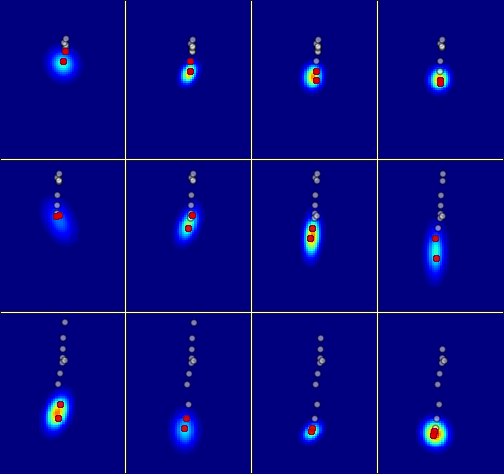
\includegraphics[width=0.45\textwidth]{figures/trajectory_pred.png}
	\end{center}
	\caption{\textbf{Trajectory prediction.} Shown is the current and past positions of the person (grey), the positions in the next two frames (red) and the prediction in the background.}
	\label{fig:trajectory_pred}
\end{figure}

\section{Conclusion}

We presented a leg and person detector, working solely on Lidar input data. Laser points are labeled with high accuracy in close range to the robot. Detecting people using the trained model is a first in neural network and we find a high precision and an overall good model. We were able to outperform the state of the art, while simultaneously needing no knowledge about people viewed from a laser sensor, their shapes and movements. From the positions of people, we are finally able to predict their trajectories, which we can use in various environments.

% needed in second column of first page if using \IEEEpubid
%\IEEEpubidadjcol

% An example of a floating figure using the graphicx package.
% Note that \label must occur AFTER (or within) \caption.
% For figures, \caption should occur after the \includegraphics.
% Note that IEEEtran v1.7 and later has special internal code that
% is designed to preserve the operation of \label within \caption
% even when the captionsoff option is in effect. However, because
% of issues like this, it may be the safest practice to put all your
% \label just after \caption rather than within \caption{}.
%
% Reminder: the "draftcls" or "draftclsnofoot", not "draft", class
% option should be used if it is desired that the figures are to be
% displayed while in draft mode.
%
%\begin{figure}[!t]
%\centering
%\includegraphics[width=2.5in]{myfigure}
% where an .eps filename suffix will be assumed under latex, 
% and a .pdf suffix will be assumed for pdflatex; or what has been declared
% via \DeclareGraphicsExtensions.
%\caption{Simulation Results}
%\label{fig_sim}
%\end{figure}

% Note that IEEE typically puts floats only at the top, even when this
% results in a large percentage of a column being occupied by floats.


% An example of a double column floating figure using two subfigures.
% (The subfig.sty package must be loaded for this to work.)
% The subfigure \label commands are set within each subfloat command, the
% \label for the overall figure must come after \caption.
% \hfil must be used as a separator to get equal spacing.
% The subfigure.sty package works much the same way, except \subfigure is
% used instead of \subfloat.
%
%\begin{figure*}[!t]
%\centerline{\subfloat[Case I]\includegraphics[width=2.5in]{subfigcase1}%
%\label{fig_first_case}}
%\hfil
%\subfloat[Case II]{\includegraphics[width=2.5in]{subfigcase2}%
%\label{fig_second_case}}}
%\caption{Simulation results}
%\label{fig_sim}
%\end{figure*}
%
% Note that often IEEE papers with subfigures do not employ subfigure
% captions (using the optional argument to \subfloat), but instead will
% reference/describe all of them (a), (b), etc., within the main caption.


% An example of a floating table. Note that, for IEEE style tables, the 
% \caption command should come BEFORE the table. Table text will default to
% \footnotesize as IEEE normally uses this smaller font for tables.
% The \label must come after \caption as always.
%
%\begin{table}[!t]
%% increase table row spacing, adjust to taste
%\renewcommand{\arraystretch}{1.3}
% if using array.sty, it might be a good idea to tweak the value of
% \extrarowheight as needed to properly center the text within the cells
%\caption{An Example of a Table}
%\label{table_example}
%\centering
%% Some packages, such as MDW tools, offer better commands for making tables
%% than the plain LaTeX2e tabular which is used here.
%\begin{tabular}{|c||c|}
%\hline
%One & Two\\
%\hline
%Three & Four\\
%\hline
%\end{tabular}
%\end{table}


% Note that IEEE does not put floats in the very first column - or typically
% anywhere on the first page for that matter. Also, in-text middle ("here")
% positioning is not used. Most IEEE journals use top floats exclusively.
% Note that, LaTeX2e, unlike IEEE journals, places footnotes above bottom
% floats. This can be corrected via the \fnbelowfloat command of the
% stfloats package.



%\section{Conclusion}
%\blindtext





% if have a single appendix:
%\appendix[Proof of the Zonklar Equations]
% or
%\appendix  % for no appendix heading
% do not use \section anymore after \appendix, only \section*
% is possibly needed

% use appendices with more than one appendix
% then use \section to start each appendix
% you must declare a \section before using any
% \subsection or using \label (\appendices by itself
% starts a section numbered zero.)
%


\appendices
%\section{Proof of the First Zonklar Equation}
%\blindtext

% use section* for acknowledgement
\section*{Acknowledgment}


The authors would like to thank...


% Can use something like this to put references on a page
% by themselves when using endfloat and the captionsoff option.
\ifCLASSOPTIONcaptionsoff
  \newpage
\fi



% trigger a \newpage just before the given reference
% number - used to balance the columns on the last page
% adjust value as needed - may need to be readjusted if
% the document is modified later
%\IEEEtriggeratref{8}
% The "triggered" command can be changed if desired:
%\IEEEtriggercmd{\enlargethispage{-5in}}

% references section

% can use a bibliography generated by BibTeX as a .bbl file
% BibTeX documentation can be easily obtained at:
% http://www.ctan.org/tex-archive/biblio/bibtex/contrib/doc/
% The IEEEtran BibTeX style support page is at:
% http://www.michaelshell.org/tex/ieeetran/bibtex/
%\bibliographystyle{IEEEtran}
% argument is your BibTeX string definitions and bibliography database(s)
%\bibliography{IEEEabrv,../bib/paper}
%
% <OR> manually copy in the resultant .bbl file
% set second argument of \begin to the number of references
% (used to reserve space for the reference number labels box)


%\begin{thebibliography}{1}

\bibliography{lib/main}
\bibliographystyle{IEEEtran}

%\bibitem{IEEEhowto:kopka}
%H.~Kopka and P.~W. Daly, \emph{A Guide to \LaTeX}, 3rd~ed.\hskip 1em plus
%  0.5em minus 0.4em\relax Harlow, England: Addison-Wesley, 1999.

%\end{thebibliography}

% biography section
% 
% If you have an EPS/PDF photo (graphicx package needed) extra braces are
% needed around the contents of the optional argument to biography to prevent
% the LaTeX parser from getting confused when it sees the complicated
% \includegraphics command within an optional argument. (You could create
% your own custom macro containing the \includegraphics command to make things
% simpler here.)
%\begin{biography}[{\includegraphics[width=1in,height=1.25in,clip,keepaspectratio]{mshell}}]{Michael Shell}
% or if you just want to reserve a space for a photo:

%\begin{IEEEbiography}[{\includegraphics[width=1in,height=1.25in,clip,keepaspectratio]{picture}}]{John Doe}
%\blindtext
%\end{IEEEbiography}

% You can push biographies down or up by placing
% a \vfill before or after them. The appropriate
% use of \vfill depends on what kind of text is
% on the last page and whether or not the columns
% are being equalized.

%\vfill

% Can be used to pull up biographies so that the bottom of the last one
% is flush with the other column.
%\enlargethispage{-5in}

% that's all folks
\ifthenelse{\equal{\paperstate}{Production}}{
	\ifnum\thecountertodo=0
	
	\else
		\clearpage
		\newpage
		\onecolumn{
		\huge IMPORTANT INFORMATION DURING PRODUCTION
		\noindent
		\normalsize \\ \\
		\ifnum\thecountertodo=1
			\noindent
			There is \arabic{countertodo} todo left!
		\else
			There are \arabic{countertodo} todos left!
		\fi
		}
	\fi
	
	\noindent
	\getabbrev{LRM}
}{}
\end{document}


